% Created 2025-10-07 Tue 10:16
% Intended LaTeX compiler: pdflatex
\documentclass[version=submission]{iacrcc}
\usepackage[utf8]{inputenc}
\usepackage[T1]{fontenc}
\usepackage{graphicx}
\usepackage{longtable}
\usepackage{wrapfig}
\usepackage{rotating}
\usepackage[normalem]{ulem}
\usepackage{amsmath}
\usepackage{amssymb}
\usepackage{capt-of}
\usepackage{alphabeta}
\usepackage{minted}
\setminted[scheme]{style=bw}
\usepackage{tikz}
\usepackage{tikz-qtree}
\usepackage{subcaption}
\newcommand{\Delete}{\mathrm{Delete}}
\newcommand{\Fetch}{\mathrm{Fetch}}
\newcommand{\Insert}{\mathrm{Insert}}
\newcommand{\Merge}{\mathrm{Merge}}
\newcommand{\Search}{\mathrm{Search}}
\newcommand{\Setup}{\mathrm{Setup}}
\newcommand{\ploc}{\text{\textsc{ploc}}}
\newcommand{\datum}{\mathrm{dat.}}
\newcommand{\cA}{\mathcal{A}}
\newcommand{\cE}{\mathcal{E}}
\newcommand{\cL}{\mathcal{L}}
\newcommand{\cN}{\mathcal{N}}
\newcommand{\cO}{\mathcal{O}}
\newcommand{\cP}{\mathcal{P}}
\newcommand{\cR}{\mathcal{R}}
\newcommand{\cS}{\mathcal{S}}
\newcommand{\cT}{\mathcal{T}}
\newcommand{\bS}{\mathbf{S}}
\newcommand{\bD}{\mathbf{D}}
\newcommand{\bbA}{\mathbb{A}}
\newcommand{\bbL}{\mathbb{L}}
\newcommand{\bbO}{\mathbb{O}}
\newcommand{\bbR}{\mathbb{R}}
\newcommand{\bbS}{\mathbb{S}}
\newcommand{\bbV}{\mathbb{V}}
\newcommand{\op}{\mathrm{op}}
\newcommand{\stt}{\mathrm{st}}
\newcommand{\args}{\mathrm{args}}
\newcommand{\res}{\mathrm{res}}
\newcommand{\spattern}{\mathrm{sp}}
\newcommand{\MM}{\mathrm{MM}}
\newcommand{\EMM}{\mathrm{EMM}}
\newcommand{\msec}{\,\mathrm{msec}}

\title{All Paths Lead to the Root}

\begin{document}
\maketitle
\begin{abstract}
  In an  attempt to fix  the defects of the  definition of forward  security for
  Symmetric     Searchable     Encryption     (SSE)    schemes,     Amjad     et
  al. \cite{AC:AmjKamMoa23}  proposed  injection  security.  This  new  security
  property is  strictly stronger  than most security  properties known  to date,
  which  makes  designing  schemes   that  meet  its  requirements  particularly
  challenging.   In this  work, we  show  how it  is  possible to  use trees  to
  decorrelate the  modification of  an index from  its effects,  hence achieving
  injection  security.  In  addition to  being conceptually  simple, our  scheme
  features non-interactive,  stateless and mutation-free search  operations that
  allow supporting  concurrent readers easily.  Finally,  the proposed reference
  implementation  is  efficient:  both \(\Insert\)  and  \(\Search\)  operations
  execute in milliseconds even  when operating on an index with  up to a million
  entries and volumes up to a thousand.
\end{abstract}


\section{Introduction}
\label{sec:org9e388b6}

Symmetric Searchable Encryption (SSE) is a  formalism used to study the security
of protocols manipulating an index stored by  a distant server: an SSE scheme is
a bipartite  protocol between a client  and an adversarial server  usually being
considered honest-but-curious. The  security an SSE scheme relies  on the notion
of  leakage to  capture the  amount  of information  the server  can acquire  by
observing the  execution of scheme  operations.  There exists a  natural tension
between the  efficiency of a  scheme and  its security.  SSE  schemes resolutely
fall into the practical side when compared to more secure schemes like ORAM, but
successive  innovations have  led to  constructions proposing  stronger security
guaranties to the  detriment of performance.  We stress that  in many real-world
applications, the performance of a scheme is almost as important as its security
since poor performances  hinder adoption, resulting in  essentially no security.
In particular, while  server-side memory is generally not  an issue, client-side
memory  is a  particularly constrained  resource.  However,  apart from  notable
works like \cite{NDSS:DCPP20}, most SSE schemes  have a space complexity that is
linear in  the number of indexed  labels \(L\).  Another source  of inefficiency
that runs even deeper into the  SSE literature is the single-client setting that
was adopted  by the founding  works and based on  which has been  formalized the
security model  most later works  adopt.  Most  SSE schemes where  thus designed
with this model  in mind and rely  on some mutable client-side  state that makes
them incompatible  with the multi-client  setting.  Some recent  developments in
\cite{AC:AgaKamMoa24,EPRINT:BreHeb24}   made  a   step  in   the  direction   of
formalizing  security in  the concurrent  setting,  but --  to the  best of  our
knowledge --  no SSE  scheme with a  decent security has  ever proved  secure in
those models.   In this  work, we  propose an  SSE scheme  with non-interactive,
stateless  and  mutation-free  search  operations   that  make  it  amenable  to
concurrent  search queries  provided the  server guarantees  basic shared-object
properties.  We  believe our scheme  opens up a  broad range of  applications in
which lightweight clients query an index managed by one powerful client.

On   the   security   front,   forward    security   --   formalized   by   Bost
in \cite{10.1145/2976749.2978303} as the unlinkability  of updates with previous
operations -- has  been considered as a state-of-the-art  security property even
though it does not guarantee that future search queries cannot be linked to past
updates.  A  persistent adversary thus  eventually learns what  forward security
attempts to hide.  Injection Security is  a much stronger property -- defined as
the unlinkability of  updates with all other past and  future operations -- that
has recently  been proposed \cite{AC:AmjKamMoa23}  to remedy  forward security's
shortcomings. We believe it  to be a real step forward, which  is why we present
in this work a new injection-secure SSE scheme named \(\ploc\).

\subsection{Related works}
\label{sec:orgc4b0537}

The first  and only  injection-secure SSE  scheme to  date \cite{AC:AmjKamMoa23}
relies on a temporal decorrelation of the modifications from their side-effects:
upon modifying bindings for a label \(\ell\), the client saves this modification
locally under  this label and performs  instead the modifications saved  under a
different label  \(\ell'\) chosen independently  from \(\ell\). In  their scheme
the authors used  a round-robin strategy going through all  the labels by batch.
The  server-side   labels  are  therefore  updated   every  \(\frac{|\bbL|}{C}\)
modifications, where \(\bbL\)  is the labeling domain and \(C\)  the batch size.
Conversely, the size of the  client-side state is \(O(\frac{|\bbL|}{C})\) in the
worst case.  The key  is to always perform the same  number of modifications per
label to avoid leaking any information on the past modifications, which requires
the client to  sometimes perform dummy modifications and results  in a bandwidth
of \(O(C \times S)\) for some constant \(S\) chosen at setup.  Conscious of this
cost, the authors astutely pad and truncate the set of values indexed under each
label to  enable users to choose  \(S = (1 -  \epsilon) \cdot V\) for  some loss
parameter \(0  < \epsilon  \le 1\)  and \(V\)  an upper-bound  on the  number of
values indexed  per label, also  chosen at setup.   However, the loss  cannot be
increased past  a certain amount  without severely damaging the  search results,
and  the bandwidth  cost remains  \(O(C \times  V)\).  The  users are  therefore
caught in  an impossible dilemma: they  must constrain the size  of the labeling
domain to limit  both the client-side stash and insertion  bandwidth at the risk
of speeding-up query-recovery attacks (since the  labels are fewer, it is easier
to tell  them apart),  or otherwise  choose between an  acceptable bound  on the
client-side storage or the bandwidth.  Finally,  since the very security of this
scheme  relies on  delaying  the  modification of  the  server  state, it  seems
impossible to use it as a basis on which to develop a concurrent SSE scheme with
anything  but  a very  relaxed  concurrency  model.   All  in all,  this  scheme
represents  a  break-through in  the  field,  but  presents  costs that  may  be
prohibitively high for many use-cases.

Even though not achieving injection  security (nor forward security), we quickly
present  here \(2ch\) \cite{PoPETS:APPYY23}  since it  is conceptually  close to
ours. This scheme is based on a  complete binary tree, in which indexing a value
under a  label consists in deriving  two candidate branches from  this label and
its current volume using  a PRF. The client then fetches  those two branches and
stores the new value inside the least filled one. Search operations always fetch
\(2V\) branches which first \(2\nu(\ell)\) correspond to the branches derived to
bind values to this  label so far, where \(\nu(\ell)\) is  the current volume of
the   label   \(\ell\).    Using    this   technique   allows   implementing   a
volume-hiding \cite{10.1145/3319535.3354213} scheme.   The authors  also managed
to reduce the bandwidth from \(O(\log B)\)  to \(O(\log \log B)\) where \(B\) is
the maximum number of bindings that can  be indexed in the tree by beheading the
tree to  create a  forest of  trees of  depth \(\log  \log B\).   The subsequent
schemes proposed in  the same article build  on this and attempt  to recover the
forward   and   backward  securities \cite{10.1145/3133956.3133980},   but   are
sub-optimal since they require search operations to perform more work.

\subsection{Contributions}
\label{sec:org9b1ea8a}

In this  work, we  propose a  novel injection-secure  SSE scheme  that spatially
decorrelates mutations  from their  effects.  Like  in \cite{PoPETS:APPYY23}, we
rely on a tree  structure and values are stored in some  node alongside the path
leading to the leaf  selected using a PRF of the indexing  label and its current
volume. However,  since all paths  lead to  the root of  a tree, the  client can
fetch uncorrelated  branches upon insertion: as  long as it possible  to compact
the resulting  subtree enough to make  space at the  root, the new value  can be
inserted on  its target path.  Upon  search, all \(V\) branches  associated to a
label are read in order to find  the indexed values. Using this technique allows
us to build a simple SSE scheme with very desirable properties:
\begin{itemize}
\item insertions  are only  required to maintain  a \(O(L)\)  client-side state,
  where  \(L\)  is the  number  of  labels  currently  indexed, to  store  their
  associated   volumes.    This   is   a  significant   improvement   over   the
  \(O(\frac{|\bbL|}{C})\)   bound    from \cite{AC:AmjKamMoa23}.    Our   scheme
  implements     insert    operations     using    two     round    trips     of
  \(O(n c  \lg |\mathbb  V| \lg  B)\) bandwidth,  where \(n\)  is the  number of
  branches fetched  from the  tree for  compaction, \(c\)  the capacity  of each
  node, \(\mathbb  V\) the value  domain and \(B\)  the total number  of indexed
  bindings;
\item searches  need only know  the key and do  not perform any  mutation, which
  allows them to be trivially concurrent and hence to implement a single-writer,
  several-readers system  that only  leaks the search  pattern. Even  though our
  insertions cannot be used by concurrent  clients due to the mutable state that
  is the  label-volume map,  we consider  it a net  improvement over  the scheme
  proposed in the recent article  from Agarwal et al. \cite{AC:AgaKamMoa24} that
  doesn't  even  guarantee  forward  security   in  the  context  of  concurrent
  operations.  Our scheme implements search operations using a single round-trip
  and a \(O(V c \lg |\mathbb V| \lg B)\) bandwidth.
\item additionally,  we show how to  apply some of the  standard techniques from
  the  literature to  implement a  more expressive  interface, for  example that
  support deletions, and to make insertions stateless.
\end{itemize}
\section{Preliminaries}
\label{sec:orgcf278e9}
\subsection{Structured Encryption}
\label{sec:org9c11e67}

Structured Encryption (STE) was  first introduced in \cite{chase2010structured}
to allow a client  to query a data structure stored by  a server with controlled
leakages. An  STE scheme  is based  on an  Abstract Data  Type (ADT)  defined as
follows:

\begin{definition}[Abstract Data Type]
  An abstract  data type  is defined as  a pair \((\bbS,  \bbO)\) of  states and
  operations on those states every realizations  of this abstract data type must
  support.  Without loss  of generality, we constrain operations  in \(\bbO\) to
  be parameterized by  their argument and result sets \(\bbA\)  and \(\bbR\) and
  to be of type \(\bbA \times \bbS \rightarrow \bbR \times \bbS\).
\end{definition}

\begin{definition}[Structured Encryption Scheme]
Given an abstract data type \(\cT = (\bbS, \bbO)\), a \(\cT\) encryption scheme is a
bipartite protocol involving  a client and a server that  supports the following
operations:
\begin{itemize}
\item \((k, \stt; EDS) \gets \Setup(DS; )\) in which the client takes as input a valid
data structure \(DS  \in \bbS\), and at  the end of which the  client receives a
key  \(k\) and  a  state \(\stt\),  and  the server  receives  the encrypted  data
structure \(EDS\) corresponding to \(DS\);
\end{itemize}
for each operation \(\op \in \bbO\) parameterized by \(\bbA\) and \(\bbR\):
\begin{itemize}
\item \((\res, \stt'; EDS') \gets \op(k, \args, \stt; EDS)\) in which the client
  takes  as  input   the  key  \(k\),  a  state  \(\stt\)   and  some  arguments
  \(\args \in  \bbA\), the  server takes  as input  an encrypted  data structure
  \(EDS\) corresponding to  a data-structure \(DS \in \bbS\), and  at the end of
  which  the client  receives  a result  \(\res  \in \bbR\)  and  the server  an
  encrypted  data  structure  \(EDS'\)   corresponding  to  the  data  structure
  \(DS'  \in \bbS\),  where  \(\res\)  and \(DS'\)  correspond  to what  locally
  applying \(\op\) on \(\args\) and \(DS\) would return.
\end{itemize}
\end{definition}

\begin{remark}
  Even though the standard definition for a structured encryption scheme expects
  the setup to take as argument  an initial data structure, the scheme described
  in this article does not. However, it is easy to see that an alternative setup
  procedure  taking as  argument a  data structure  can be  obtained while  only
  leaking  its  size  by executing  a  setup  followed  by  one or  more  update
  operations without any additional leakage since the \(\ploc\) insert operation
  only has a trivial leakage.
\end{remark}
\subsection{Multi-map Encryption Scheme}
\label{sec:orgcc2afca}

One particular instance of structured encryption  has been at the center of most
of the  works in the literature  for its immediate applicability:  the multi-map
encryption scheme.

\begin{definition}[Multi-Map]
  A (semi-dynamic) multi-map  is an abstract data type parameterized  by a label
  domain  \(\bbL\) and  a  value domain  \(\bbV\), which  valid  states are  the
  functions       in       \(\bbL        \rightarrow       \bbV^*\),       where
  \(\bbV^* = \bot  \cup \left(\bbV \times \bbV^*\right)\),  and which operations
  are:
  \begin{itemize}
  \item \(((v_i)_i,  \MM) \gets \Search(\ell,  \MM)\) takes as argument  a label
    \(\ell\) and a valid state \(\MM\), and returns the (possibly empty) list of
    values bound to that label by the given state;
  \item \((\bot, \MM') \gets \Insert((\ell, v), \MM)\) takes as argument a label
    \(\ell \in \bbL\), a  value \(v \in \bbV\) and a  state \(\MM\), and returns
    the new state \(\MM'\) such that \(\MM'(\ell') = \MM(\ell')\) for each label
    \(\ell' \ne \ell\) and \(\MM'(\ell) = (v, \MM(\ell))\) otherwise.
  \end{itemize}
  A multi-map is said to be fully-dynamic if it additionally supports:
  \begin{itemize}
  \item \((\bot, \MM') \gets \Delete((\ell, v), \MM)\) takes as argument a label
    \(\ell \in \bbL\), a  value \(v \in \bbV\) and a  state \(\MM\), and returns
    the new state \(\MM'\) such that \(\MM'(\ell') = \MM(\ell')\) for each label
    \(\ell' \ne \ell\) and \(\MM'(\ell) = \MM(\ell) \setminus \ell\) otherwise.
  \end{itemize}
\end{definition}

\begin{definition}[Multi-Map Encryption Scheme]
  A  (semi-dynamic)  multi-map  encryption  scheme  is  therefore  the  protocol
  parameterized  by   an  label  domain   \(\mathbb  L\)  and  a   value  domain
  \(\mathbb V\) that  exposes the following operations which  semantics is given
  by the STE definition:
\begin{itemize}
\item \(((v_i)_i, \stt'; \EMM) \gets \Search(k, \ell, \stt; \EMM)\);
\item \((\bot, \stt'; \EMM') \gets \Insert(k, (\ell, v), \stt; \EMM)\).
\end{itemize}
A multi-map  encryption scheme is  said to  be fully-dynamic if  it additionally
exposes:
\begin{itemize}
\item \((\bot, \stt'; \EMM') \gets \Delete(k, (\ell, v), \stt; \EMM)\).
\end{itemize}
\end{definition}
\subsection{Symmetric Searchable Encryption}
\label{sec:org1e69724}

While structured  encryption addresses the  abstract and fundamental  problem of
securing  data-structures, Symmetric  Searchable Encryption  (SSE) as  described
in \cite{10.1145/1180405.1180417} by  Curtmola et al. addresses  the problem of
securing a specific  use-case in which a  client wishes to retrieve  the list of
document  IDs of  all documents  matching a  given label,  from a  collection of
documents   stored  in   a   remote  server.    While   the  interface   defined
in \cite{10.1145/1180405.1180417}  differs from  those  of a  multi-map, it  is
trivial to implement an SSE scheme  from a multi-map encryption scheme. For this
reason, we claim in this work to  present a new SSE scheme while only presenting
a new encrypted multi-map implementation.
\subsection{Leakages and adaptive security}
\label{sec:org97fc2a5}

The leakage function plays a central role in the SSE literature since it is used
to quantify the information leaked to  the adversary by each operation.  In this
work, we consider the notion  of adaptive security against a honest-but-curious,
polynomial-time server.

\begin{definition}
An STE scheme \(\Sigma\) is said to be \(\cL\)-adaptively-secure if there exists a
simulator \(\phi\)  such that  for any  stateful honest-but-curious  PPT adversary
\(\cA\)   and   any   auxiliary    information   \(z   \in   \{0,1\}^*\):   \[\left|
P(\mathbf{Real}_{\Sigma,\cA}(1^\lambda,  z)  =  1)  -  P(\mathbf{Ideal}_{\Sigma,
\cA}^{\phi, \cL}(1^\lambda, z)  = 1) \right| =  \mathtt{negl}(\lambda), \] where
the real and ideal games are defined as follows:
\begin{itemize}
\item the challenger  either executes  the client  code of  the STE  scheme \(\Sigma\)
(real game)  or the  composition \(\phi  \circ \cL\) of  the simulator  with the
leakage function  (ideal game), while the  adversary plays the server  code of
the STE scheme \(\Sigma\).
\item the  adversary  adaptively  chooses  a   sequence  of  (polynomially  many  in
\(\lambda\)) ADT operations that are jointly executed with the challenger.
\item the adversary outputs a bit \(b\in \{0,1\}\).
\end{itemize}
\end{definition}
\subsection{Security properties}
\label{sec:org11304b1}

If leakage functions capture the information that is leaked by SE operations,
evaluating the level of privacy guaranteed by a given leakage or even
establishing an order relation on the leakages that reflects those security
guarantees remains a difficult
problem \cite{PoPETS:BosFou19}\cite{10.1145/3548606.3560593}.  It has thus
become idiomatic to describe scheme privacy using \emph{security properties},
which are associated to the set of attacks known to hold against them.

The most important  source of attacks against SSE schemes  is the search pattern
-- sometimes called  query equality -- which  allows an attacker to  partition a
sequence of  search queries with respect  to the searched label  (without always
being able to guess which are those labels).

\begin{definition}[Search Pattern]
Given a sequence of \(m\) search operations \((o_1, ..., o_m)\), the search pattern,
noted \(\spattern\), is the matrix \(M \in \{0,1\}^{m \times m}\) such that \(M[i][j]
= i\)  if and only  if the operations  \(o_i\) and \(o_j\)  both search for  the same
label.
\end{definition}

\begin{remark}
If the  label domain \(\bbL\)  is countable, there  exists a bijection  \(idx\) from
\([0,|\bbL|[\) to \(\bbL\) and the matrix-based  definition of the search pattern is
equivalent   to  leaking   \(\pi_{[0,|\bbL|[}  \circ   idx^{-1}  (\ell)\),   where
\(\pi_{[0,|\bbL|[}\) is a random permutation  on \([0,|\bbL|[\).  This definition is
easier to use in practice since it is comes up more naturally in the proofs.
\end{remark}

Injection  security  is  a  property  of  the  leakage  functions  of  multi-map
encryption  schemes that  has  recently  been defined  in \cite{AC:AmjKamMoa23}
guaranteeing that  no link  can ever  be made between  a mutation  (insertion or
deletion) and any other past or future  operation.  While we refer the reader to
the original article for its game-based  definition, we give here the sufficient
condition we use in this article:

\begin{theorem}[Injection Security]
A leakage  function \(\cL\) is said  to be injection-secure if  \(\cL(\op, \args) =
(\op, \spattern)\) if \(\op\) is \(\Search\) and \(\op\) otherwise.
\end{theorem}

\begin{proof}
See the proof of Theorem 3.3 from \cite{AC:AmjKamMoa23}.
\end{proof}
\subsection{Notations}
\label{sec:orgd3df2ea}

In the rest of this article, we make use of the notations listed in
table \ref{tab:org8d282d4}.

\begin{table}[htbp]
\caption{\label{tab:org8d282d4}Notations used in this article.}
\centering
\begin{tabular}{|l|l|}
\hline
notation & description\\
\hline
\(s\) & node size\\
\(c\) & node capacity\\
\(\ell\) & label\\
\(v\) & value\\
\(d\) & depth\\
\(n\) & number of branches selected for compaction\\
\(B\) & upper-bound on the number of bindings\\
\(L\) & upper-bound on the number of labels\\
\(N\) & upper-bound on the number of tree leaves\\
\(V\) & upper-bound on the maximum label volume\\
\(\phi\) & \((s,D)\)-tree-encryption-scheme simulator\\
\(\psi\) & \(\ploc\) simulator\\
\hline
\end{tabular}
\end{table}
\section{Description}
\label{sec:orgf23ee2f}

The complete algorithm is given in appendix \ref{sec:org8180c74}. We have chosen
to implement it in the Scheme programming language \cite{10.5555/1618542} for
its well-defined semantics and conciseness\footnote{The entire reference
  implementation given in appendix \ref{sec:orgeb8c851} is less than 400 lines
  long.}, which incidentally provides a reference implementation for \(\ploc\).
A description of the syntax required to understand this code is provided in
appendix \ref{sec:org41ce977}.  The present section details the most important
aspects of the algorithm step by step.  It is assumed that the following names
are in scope:
\begin{itemize}
\item \texttt{c} the capacity of each node (i.e. the maximum number of datums they can
store);
\item \texttt{n} the number of branches to compact per insertion;
\item \texttt{B} the maximum number of bindings allowed;
\item \texttt{V} the maximum volume allowed;
\item  \texttt{(H key  label volume)}  a cryptographic  hash function  taking as
  input a 128-bit key, a label bit-string  of arbitrary size and an integer, and
  produces a  128-bit integer.  Its  only required  security guarantee is  to be
  indistinguishable from a pseudo-random function;
\end{itemize}
Since  \(\ploc\) is  based on  a complete  binary tree,  we introduce  here some
vocabulary used to describe trees.  A \emph{branch} is defined as the bit-string
representing the choices to be made at each level between the left and the right
children of a node. This bit-string is encoded as an integer in which the choice
made  at the  root is  encoded by  the  bit of  exponent zero.   This choice  of
representation allows for efficient and  simple tree traversals.  A branch needs
not be smaller that \(N\) since the  bits following the first \(\lg N\) ones are
ignored by the traversal.  This allows using the output of \texttt{H} as branch.
The \emph{ID} of  a given node at depth  \(d\) is the prefix of  length \(d\) of
any  branch  to  which  this  node  belongs:  it  is  therefore  the  bit-string
representing the sequence  of choices made at  each level from the  root to that
node, encoded as an integer the same way a branch is.

To   manipulate   this   complete   binary   tree,   \(\ploc\)   relies   on   a
\((s,  N)\)-complete-binary-tree encryption  scheme  defined  as the  structured
encryption scheme based on the ADT parameterized by \(s\) and \(N\), which valid
states are the  complete binary trees of  \(N\) leaves and nodes  of size \(s\),
and which operations are:
\begin{itemize}
\item \((t, T')  \gets \Fetch(\mathrm{branches}, T)\), that  returns the subtree
  \(t\) defined by the given branches in \(T\);
\item \((\bot, T') \gets \Merge(t, T)\) that merges the given subtree \(t\) with
  the tree \(T\) by replacing all tree  nodes by their equivalent in the subtree
  when it exists.
\end{itemize}
An implementation of such a scheme is given in appendix \ref{sec:org460d7e4}.

\subsection{Setup procedure}
\label{sec:orgac56433}

The setup simply consists in initializing the tree encryption scheme:
\begin{minted}[]{scheme}
(define (ploc-setup) (tree-setup))
\end{minted}
\subsection{Insertion procedure}
\label{sec:orgcade814}

In \(\ploc\) as in most SSE, inserting requires the client to store the volumes of
each label. This can be done using a hash map:
\begin{minted}[]{scheme}
(define volumes (make-hmap))

(define (get-volume label)
  (hmap-find volumes label 0))

(define (increment-volume label)
  (let ((volume (get-volume label)))
    (hmap-bind! volumes label (+ volume 1))))
\end{minted}
Each binding is stored wrapped inside a \emph{datum} that holds both the indexed
value, and a \emph{target} branch.
\begin{minted}[]{scheme}
(define (new-datum target value) (vector target value))

(define (datum->target datum) (vector-ref datum 0))
(define (datum->value  datum) (vector-ref datum 1))
\end{minted}
The target is a pseudo-random number computed using the cryptographic hash \texttt{H}
and the \texttt{key}.
\begin{minted}[]{scheme}
(define (get-target key label volume)
  (H key label volume))
\end{minted}
\begin{minted}[]{scheme}
(define (make-datum key label value)
  (let* ((volume (get-volume label))
         (target (get-target key label volume)))
    (new-datum target value)))
\end{minted}
Storing  the  target  branch  in  each datum  enables  future  modifications  to
\emph{compact} the tree while  maintaining the invariant \emph{(\textbf{I}) each
  datum is on  its target branch}, and the  post-condition \emph{(\textbf{P}) no
  datum can be pushed further down}.

The compaction is performed on a subtree  extracted from the main tree using the
\texttt{tree-fetch} procedure.   The branches  used to  select this  subtree are
generated  using a  procedure of  no argument  called a  \emph{scheduler}.  Some
scheduling  strategies are  better  than others.   Indeed, if  the  same set  of
branches were to be constantly scheduled for compaction, the datums which target
branches have  a small intersection with  this set of branches  would accumulate
near the root of the tree, eventually causing an overflow. We therefore choose a
scheduling strategy that sweeps the tree  branches in a regular and uniform way:
each  lower-bit combination  is covered  by a  single selected  branch, and  all
selected branches circle the higher-bit combinations in a circular fashion.  For
example  with  $N=8$  and  $n=2$,  all nodes  from  the  two  upper-most  levels
representing  the two  lowest  bits are  covered.   Then, at  each  call to  the
scheduler, these  bits are prepended  the bits  generated by selecting  the next
integer  modulo   $\frac{N}{n}=4$,  resulting   in  the  subtrees   depicted  in
Figure \ref{fig:scheduling}.
\begin{figure}[h]
  \centering
\begin{tabular}{cc}
\includegraphics{img/tree-1.pdf}
&
\includegraphics{img/tree-2.pdf}
\\
$t=0$ & $t=1$
\\
&
\\
\includegraphics{img/tree-3.pdf}
&
\includegraphics{img/tree-4.pdf}
\\
$t=2$ & $t=3$
\\
\end{tabular}
\caption{Scheduling cycle for $N=8$ and $n=2$.\label{fig:scheduling}}
\end{figure}
The following \texttt{make-scheduler} procedure  generates a stateful scheduler drawing
batches of \texttt{n} branches.
\begin{minted}[]{scheme}
(define (make-scheduler n)
    (assert (integer? (lg n)))
    (let ((counter 0) (prefixes (iota n)))
      (λ ()
        (set! counter (+ counter 1))
        (map (λ (pfx) (+ pfx (* counter n)))
             prefixes))))
\end{minted}
\begin{minted}[]{scheme}
(define scheduler (make-scheduler n))
\end{minted}
The compaction is a recursive procedure:  it accumulates the data targeting each
leaf on its way  down, and stores it back to the tree  on its way up, saturating
the  nodes  with  the  \texttt{c}  first remaining  datums  selected  using  the
following \texttt{take} procedure.
\begin{minted}[]{scheme}
(define (take n xs)
  (let loop ((n n) (xs xs) (taken (list)))
    (if (or (zero? n) (null? xs))
        (values taken xs)
        (loop (- n 1) (cons (head xs) taken) (tail xs)))))
\end{minted}
At each  level, to tell  apart data targeting the  left and right  subtrees, the
procedure \texttt{(split-with  pred? xs)}  is used.  It  returns two  lists: one
containing values that  match the given predicate and one  containing those that
don't.
\begin{minted}[]{scheme}
(define (split-with pred? xs)
  (let loop ((xs xs) (lhs (list)) (rhs (list)))
    (match xs
      ((x . xs) (if (pred? x)
                    (loop xs (cons x lhs) rhs)
                    (loop xs lhs (cons x rhs))))
      (()       (values lhs rhs)))))
\end{minted}
The predicate  \texttt{(go-left? depth branch)}  returns whether the choice  encoded at
the given depth in the given branch is to select the left child.
\begin{minted}[]{scheme}
(define (go-left? depth branch)
  (zero? (&& (<< 1 depth) branch)))
\end{minted}
\begin{minted}[]{scheme}
(define (compact node depth data)
  (define (left-datum? datum)
    (go-left? depth (datum->target datum)))
  (define (direct-data data)
    (split-with left-datum? data))
  (match node
    (#(node-data l-child r-child)
     (let*-values
         (((l-data  r-data) (direct-data (append node-data data)))
          ((l-child l-data) (compact l-child (+ depth 1) l-data))
          ((r-child r-data) (compact r-child (+ depth 1) r-data))
          ((node-data rest) (take c (append l-data r-data))))
       (values (make-node node-data l-child r-child) rest)))
    (_ (values node data))))
\end{minted}
The preservation  of the invariant (\textbf{I})  can be proven by  recurrence by
showing that a datum  is accumulated up to the last node  in the intersection of
its  target  branch  with  the  fetched  subtree.   This  proof  relies  on  the
correctness of  the \texttt{left-datum?} and \texttt{split-with}  procedures and
the use of sentinel nodes that make processing the last node of the intersection
like any other node. Once this is  done, the rest of the proof follows trivially
since the nodes in which a datum can be placed back are the nodes visited during
the  recursive   calls  which  have  been   proven  to  belong  to   its  target
branch.  Proving (\textbf{P})  is simple  since the  backtracking saturates  the
lower nodes first, until there is no datum left or the tree overflows.

In order to insert a new datum, \(\ploc\) simply calls the compaction procedure on
the next scheduled subtree with this datum.
\begin{minted}[]{scheme}
(define (ploc-insert key label value)
  (let ((data    (list (make-datum key label value)))
        (subtree (tree-fetch key (scheduler))))
    (let-values (((subtree data) (compact subtree 0 data)))
      (unless (null? data)
        (error "tree overflow" subtree label value))
      (increment-volume label)
      (tree-merge key subtree))))
\end{minted}
We  conclude   this  section   with  the   graphical  representation   given  in
Figure \ref{fig:compaction}  of  the  compaction  process  focused  on  a  datum
inserted  at \(t=0\)  (for the  sake  of clarity,  the  tree is  supposed to  be
initially empty and the datums inserted at \(t=1,2,3\) are not represented).

\begin{figure}[h]
  \centering
\begin{tabular}{cc}
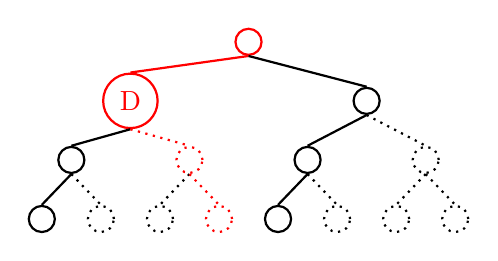
\begin{tikzpicture}[thick, scale=.5,
  level 1/.style={sibling distance=6cm},
  level 2/.style={sibling distance=3cm},
  level 3/.style={sibling distance=1.5cm}]
  \node [draw, circle] {} [red]
  child { node [draw, circle] { D }
    child [black] { node [draw, circle] {}
      child { node [draw, circle] {} }
      child [dotted] { node [draw, circle] {} }
    }
    child [dotted] { node [draw, circle] {}
      child [black] { node [draw, circle] {} }
      child { node [draw, circle] { } }
    }
  }
  child [black] { node [draw, circle] {}
    child { node [draw, circle] {}
      child { node [draw, circle] {} }
      child [dotted] { node [draw, circle] {} }
    }
    child [dotted] { node [draw, circle] {}
      child { node [draw, circle] {} }
      child { node [draw, circle] {} }
    }
  }
  ;
\end{tikzpicture}
&
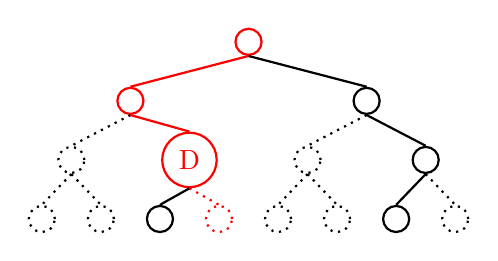
\begin{tikzpicture}[thick, scale=.5,
  level 1/.style={sibling distance=6cm},
  level 2/.style={sibling distance=3cm},
  level 3/.style={sibling distance=1.5cm}]
  \node [draw, circle] {} [red]
  child { node [draw, circle] {}
    child [dotted, black] { node [draw, circle] {}
      child { node [draw, circle] {} }
      child { node [draw, circle] {} }
    }
    child { node [draw, circle] { D }
      child [black] { node [draw, circle] {} }
      child [dotted] { node [draw, circle] { } }
    }
  }
  child [black] { node [draw, circle] {}
    child [dotted] { node [draw, circle] {}
      child { node [draw, circle] {} }
      child { node [draw, circle] {} }
    }
    child { node [draw, circle] {}
      child { node [draw, circle] {} }
      child [dotted] { node [draw, circle] {} }
    }
  }
  ;
\end{tikzpicture}
\\
$t=0$ & $t=1$
\\
&
\\
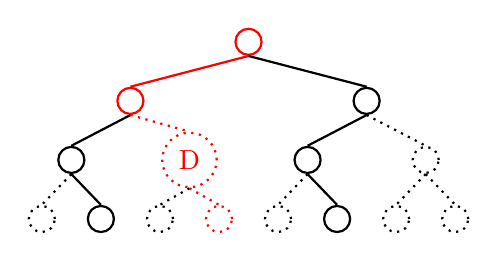
\begin{tikzpicture}[thick, scale=.5,
  level 1/.style={sibling distance=6cm},
  level 2/.style={sibling distance=3cm},
  level 3/.style={sibling distance=1.5cm}]
  \node [draw, circle] {} [red]
  child { node [draw, circle] {}
    child [black] { node [draw, circle] {}
      child [dotted] { node [draw, circle] {} }
      child { node [draw, circle] {} }
    }
    child [dotted] { node [draw, circle] { D }
      child [black] { node [draw, circle] {} }
      child { node [draw, circle] { } }
    }
  }
  child [black] { node [draw, circle] {}
    child { node [draw, circle] {}
      child [dotted] { node [draw, circle] {} }
      child { node [draw, circle] {} }
    }
    child [dotted] { node [draw, circle] {}
      child { node [draw, circle] {} }
      child { node [draw, circle] {} }
    }
  }
  ;
\end{tikzpicture}
&
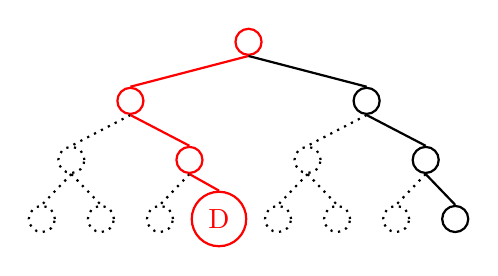
\begin{tikzpicture}[thick, scale=.5,
  level 1/.style={sibling distance=6cm},
  level 2/.style={sibling distance=3cm},
  level 3/.style={sibling distance=1.5cm}]
  \node [draw, circle] {} [red]
  child { node [draw, circle] {}
    child [dotted, black] { node [draw, circle] {}
      child { node [draw, circle] {} }
      child { node [draw, circle] {} }
    }
    child { node [draw, circle] {}
      child [dotted, black] { node [draw, circle] {} }
      child { node [draw, circle] { D } }
    }
  }
  child [black] { node [draw, circle] {}
    child [dotted] { node [draw, circle] {}
      child [dotted] { node [draw, circle] {} }
      child { node [draw, circle] {} }
    }
    child { node [draw, circle] {}
      child [dotted] { node [draw, circle] {} }
      child { node [draw, circle] {} }
    }
  }
  ;
\end{tikzpicture}
\\
$t=2$ & $t=3$
\\
\end{tabular}
\caption{Four consecutive insertions cooperating to push a datum ($D$) down its
  target path (in red) for $N=8$ and $n=2$ (compacted subtrees in plain).
  \label{fig:compaction}}
\end{figure}

\subsection{Search procedure}
\label{sec:org2b0fb59}

The search  procedure is much simpler:  it fetches the subtree  generated by all
branches possibly targeted by values indexed under the searched label,
\begin{minted}[]{scheme}
(define (get-all-targets key label)
  (map (λ (v) (get-target key label v))
       (iota V)))
\end{minted}
and for  each target branch,  filters out data  that doesn't target  the correct
label.
\begin{minted}[]{scheme}
(define (find-data subtree target)
  (define (matching-datum? datum)
    (= (datum->target datum) target))
  (filter matching-datum? (branch-data subtree target)))
\end{minted}
Only  one datum  per  target  should be  found  since  \texttt{target} contains  enough
entropy.
\begin{minted}[]{scheme}
(define (ploc-search key label)
  (let* ((targets  (get-all-targets key label))
         (subtree  (tree-fetch key targets)))
    (foldl (λ (result target)
             (match (find-data subtree target)
               (()      result)
               ((datum) (cons (datum->value datum) result))
               ( data   (error ploc-search
                               "more than one datum found"
                               data))))
           (list)
           targets)))
\end{minted}

\section{Security analysis}
\label{sec:org6cf3c32}

In this section,  we assume the existence  of a \(\cL_{\tau}\)-adaptively-secure
\((s, N)\)-tree encryption scheme, where \(\cL_\tau\) is defined as follow:
\begin{itemize}
\item \(\cL_{\tau}(\Setup) = \Setup\);
\item \(\cL_{\tau}(\Fetch, \{b_i\}) = (\Fetch, \{b_i\})\);
\item \(\cL_{\tau}(\Merge, \mathrm{subtree}) = (\Merge, \{b_i\})\).
\end{itemize}
That is, the  tree encryption scheme operations only leak  the branches defining
the subtree they are working on.  Such  a scheme is actually trivial to designed
and one possible implementation is described in section \ref{sec:org460d7e4}.

\begin{theorem}
Given a \(\cL_{\tau}\)-adaptively-secure \((s,  N)\)-tree encryption scheme with
public  parameters  \(pp_{\tau}\),  \(\ploc\) is  a  \(\cL_{\pi}\)-adaptively-secure
\((\bbL,\bbV)\)-multi-map encryption scheme  with public parameters \((pp_{\tau},
c,  n, B,  V)\), where  \(s =  c\lg|\bbV|\), \(N=B\)  and \(\cL_{\pi}\)  is defined  as
follows:
\begin{itemize}
\item \(\cL_{\pi}(\Setup) = \Setup\)
\item \(\cL_{\pi}(\Search, \ell) = (\Search, \spattern)\)
\item \(\cL_{\pi}(\Insert, \ell, v) = \Insert\)
\end{itemize}
\end{theorem}

\begin{proof}
Given the  domain \(\bbL\) and codomain  \(\bbV\), the public parameters  \((c, n, B,
V)\), and a  \(\cL_{\tau}\)-adaptively-secure \((c\lg|\bbV|, B)\)-tree encryption
scheme   with   public   parameters   \(pp_\tau\),  there   exists   a   simulator
\(\phi_{pp_\tau}\)    such    that    \(\phi_{pp_\tau}   \circ    \cL_{\tau}\)    is
indistinguishable  from  a  legitimate   tree-encryption-scheme  client  in  the
security  game given  in  \ref{sec:org97fc2a5}.   In the  following
sections, we show how to build  a simulator \(\psi^{pp_{\tau}}_{c, n, B, V}\) such
that \(\psi^{pp_{\tau}}_{c, n,  B, V} \circ \cL_\pi\) is  indistinguishable from a
legitimate \(\ploc\) client in  the same game.
\end{proof}

Note that in the implementation  given in section \ref{sec:org460d7e4}, the only
public parameter of the tree encryption-scheme is the encryption overhead.

\begin{corollary}
Given a \(\cL_{\tau}\)-adaptively-secure \((s,  N)\)-tree encryption scheme with
public    parameters    \(pp_{\tau}\),     \(\ploc\)    is    an    injection-secure
\((\bbL,\bbV)\)-multi-map encryption scheme  with public parameters \((pp_{\tau},
c, n, B, V)\), where \(s = c\lg|\bbV|\), \(N = B\).
\end{corollary}

\begin{proof}
Direct using the sufficient condition from \cite{AC:AmjKamMoa23}.
\end{proof}
\subsection{Setup}
\label{sec:org302f74d}

Recall the \(\ploc\) setup simply calls the  tree setup, which only leaks the name
of the operation:
\begin{minted}[]{scheme}
(define (psi-setup) (phi 'setup))
\end{minted}
Therefore, a \(\ploc\) setup only has trivial leakages:
\(\cL_\pi(\Setup) = \Setup.\)
\subsection{Search}
\label{sec:org72bac73}

In a nutshell, the only client-server interaction performed by a search consists
in fetching  the subtree targeted  by the  searched label.  In  particular, this
subtree does  not depend on  the volume of  this label but  on \(V\) which  is a
public \(\ploc\) parameter.  Then, by security  of the tree scheme, reading this
subtree only leaks the branches that generate  it, which in turn only depends on
the search pattern which is therefore the only non-trivial leakage.

Recall the search operation works as follows:
\begin{minted}[]{scheme}
(define (get-target key label volume)
  (H key label volume))

(define (get-all-targets key label)
  (map (λ (v) (get-target key label v))
       (iota V)))

(define (find-data subtree target)
  (define (matching-datum? datum)
    (= (datum->target datum) target))
  (filter matching-datum? (branch-data subtree target)))

(define (ploc-search key label)
  (let* ((targets  (get-all-targets key label))
         (subtree  (tree-fetch key targets)))
    (reverse
     (foldl (λ (result target)
              (match (find-data subtree target)
                (()      result)
                ((datum) (cons (datum->value datum) result))
                ( data   (error ploc-search
                                "more than one datum found"
                                data))))
            (list)
            targets))))
\end{minted}
Ignoring the fetched tree does not leak any information:
\phantomsection
\label{orge65f66b}
\begin{verbatim}
@@ -5,21 +5,7 @@
   (map (λ (v) (get-target key label v))
        (iota V)))

-(define (find-data subtree target)
-  (define (matching-datum? datum)
-    (= (datum->target datum) target))
-  (filter matching-datum? (branch-data subtree target)))
-
 (define (ploc-search key label)
-  (let* ((targets  (get-all-targets key label))
-         (subtree  (tree-fetch key targets)))
-    (reverse
-     (foldl (λ (result target)
-              (match (find-data subtree target)
-                (()      result)
-                ((datum) (cons (datum->value datum) result))
-                ( data   (error ploc-search
-                                "more than one datum found"
-                                data))))
-            (list)
-            targets))))
+  (let* ((targets (get-all-targets key label))
+         (subtree (tree-fetch key targets)))
+    (values)))
\end{verbatim}
In the oracle model, the keyed hash function can be replaced by a call to a PRF.
\phantomsection
\label{org9db0982}
\begin{verbatim}
@@ -1,11 +1,4 @@
-(define (get-target key label volume)
-  (H key label volume))
-
-(define (get-all-targets key label)
-  (map (λ (v) (get-target key label v))
-       (iota V)))
-
 (define (ploc-search key label)
-  (let* ((targets (get-all-targets key label))
+  (let* ((targets (map (λ (v) (PRF label v)) (iota V)))
          (subtree (tree-fetch key targets)))
     (values)))
\end{verbatim}
Then,  by security  of the  PRF,  the label  can  be replaced  by any  bijection
\(f:\mathbb{L}\rightarrow [1,|\bbL|]\),  transforming the  given \texttt{label}  into its
index \texttt{label-idx}:
\phantomsection
\label{org36e4689}
\begin{verbatim}
@@ -1,4 +1,4 @@
-(define (ploc-search key label)
-  (let* ((targets (map (λ (v) (PRF label v)) (iota V)))
+(define (ploc-search key label-idx)
+  (let* ((targets (map (λ (v) (PRF label-idx v)) (iota V)))
          (subtree (tree-fetch key targets)))
     (values)))
\end{verbatim}
By  security of  the tree  encryption scheme,  the call  to \texttt{tree-fetch}  can be
replaced   by   a   call    to   \(\phi_{pp_\tau}   \circ   \cL_{\tau}\).    Since
\(\cL_{\tau}(\Fetch,    \mathrm{targets})    =    (\Fetch,    \mathrm{targets})\),
\texttt{(tree-fetch key targets)} is indistinguishable from \texttt{(phi 'fetch targets)}:
\phantomsection
\label{org69d88a5}
\begin{verbatim}
@@ -1,4 +1,4 @@
-(define (ploc-search key label-idx)
+(define (ploc-search label-idx)
   (let* ((targets (map (λ (v) (PRF label-idx v)) (iota V)))
-         (subtree (tree-fetch key targets)))
+         (subtree (phi 'fetch targets)))
     (values)))
\end{verbatim}

\noindent
which gives:
\begin{minted}[]{scheme}
(define (psi-search label-idx)
  (let* ((targets (map (λ (v) (PRF label-idx v)) (iota V)))
         (subtree (phi 'fetch targets)))
    (values)))
\end{minted}
Therefore, the only non-trivial leakage of  a \(\ploc\) search is some indexing on
the  labels,   which  is   the  definition  of   leaking  the   search  pattern:
\(\cL_\pi(\Search, \ell) = (\Search, \spattern)\).
\subsection{Insert}
\label{sec:orga2e5299}

Recall the insertion works as follows:
\begin{minted}[]{scheme}
(define (get-target key label volume)
  (H key label volume))

(define (make-datum key label value)
  (let* ((volume (get-volume label))
         (target (get-target key label volume)))
    (new-datum target value)))

(define (ploc-insert key label value)
  (let ((data    (list (make-datum key label value)))
        (subtree (tree-fetch key (scheduler))))
    (let-values (((subtree data) (compact subtree 0 data)))
      (unless (null? data)
        (error "tree overflow" subtree label value))
      (increment-volume label)
      (tree-merge key subtree))))
\end{minted}
and suppose for now that compaction never overflows. The insertion can therefore
be reduced without adversarial advantage to a procedure that ignores compaction
error:
\phantomsection
\label{orgea71ce5}
\begin{verbatim}
@@ -9,8 +9,6 @@
 (define (ploc-insert key label value)
   (let ((data    (list (make-datum key label value)))
         (subtree (tree-fetch key (scheduler))))
-    (let-values (((subtree data) (compact subtree 0 data)))
-      (unless (null? data)
-        (error "tree overflow" subtree label value))
+    (let ((subtree (compact subtree 0 data)))
       (increment-volume label)
       (tree-merge key subtree))))
\end{verbatim}
By  security  of the  tree  encryption  scheme,  the  call to  \texttt{(tree-fetch  key
targets)} can  be replaced with  only negligible adversarial advantage  by \texttt{(phi
'fetch targets)},  and the call to  \texttt{(tree-merge key subtree)} can  similarly be
replaced by a call to \texttt{(phi 'merge targets)}.
\phantomsection
\label{orgefa8f7f}
\begin{verbatim}
@@ -7,8 +7,9 @@
     (new-datum target value)))

 (define (ploc-insert key label value)
-  (let ((data    (list (make-datum key label value)))
-        (subtree (tree-fetch key (scheduler))))
-    (let ((subtree (compact subtree 0 data)))
+  (let* ((data    (list (make-datum key label value)))
+         (targets (scheduler))
+         (subtree (phi 'fetch targets)))
+    (let ((subtree (compact subtree 0 (list datum))))
       (increment-volume label)
-      (tree-merge key subtree))))
+      (phi 'merge targets))))
\end{verbatim}
Finally, removing unused variables can be performed without adversarial
advantage:
\phantomsection
\label{org8eadf64}
\begin{verbatim}
@@ -1,15 +1,4 @@
-(define (get-target key label volume)
-  (H key label volume))
-
-(define (make-datum key label value)
-  (let* ((volume (get-volume label))
-         (target (get-target key label volume)))
-    (new-datum target value)))
-
-(define (ploc-insert key label value)
-  (let* ((data    (list (make-datum key label value)))
-         (targets (scheduler))
-         (subtree (phi 'fetch targets)))
-    (let ((subtree (compact subtree 0 (list datum))))
-      (increment-volume label)
-      (phi 'merge targets))))
+(define (ploc-insert)
+  (let ((targets (scheduler)))
+    (phi 'fetch targets)
+    (phi 'merge targets)))
\end{verbatim}
which gives:
\begin{minted}[]{scheme}
(define (psi-insert)
  (let ((targets (scheduler)))
    (phi 'fetch targets)
    (phi 'merge targets)))
\end{minted}
Therefore a \(\ploc\)  insertion only has trivial leakages if  compaction does not
overflow.  The following  section  gives  constraints on  \(c\)  to guarantee  the
absence  of overflow  with overwhelming  probability in  the security  parameter
\(\lambda\).
\subsection{Compaction overflow}
\label{sec:orgc58cad4}

We need to prove two different properties of the compaction process:
\begin{itemize}
\item a static property \(\mathbf{S}\) guaranteeing that the tree does not overflow in
its maximally compacted  state. This is a classic requirement  with which most
tree  algorithms  need  to  comply  and  has a  well  known  solution  in  the
balls-and-bins model (see for example \cite{10.1007/3-540-49543-6_13}): it is
enough to  allocate \(\frac{B}{N} + \frac{a\ln  N}{\ln \ln N}\), \(a>1\)  slots to
each leaf in order to guarantee \(\mathbf{S}\) with a probability in \(1 - o(1)\),
where \(N\) is the number of leaves in  the tree, \(B\) the total number of values
inserted (which  we shall call  bindings in  our context). However,  since the
absence of overflow is critical for the rest of the security proof to hold, we
will  need  to  work  out  the  proof  of  an  upper  bound  with  probability
\(1-2^{-\lambda}\).
\item a dynamic property \(\bD\) guaranteeing that a congestion leading to an overflow
at the  root only  happen with  a probability negligible  in \(\lambda\)  in the
worst case.  To the  best of our  knowledge, this kind  of probability  is not
standard.
\end{itemize}

First,  recall that  given a  random variable  \(X\) following  a binomial  law of
parameter        \(B\)        and        \(p\),        the        Chernoff-Hoeffding
theorem \cite{chernoff_1952,Hoeffding1963probabilityif}  allows  bounding  the
probability of the upper tail of that distribution:
\[\begin{array}{ccl}
  P(X \ge k) & \le & \exp\left(-B \cdot \mathrm{D}\left(\frac{k}{B}||p \right)\right) \\
             & \le & \left[\left(\frac{k}{Bp} \right)^{\frac{k}{B}}  \left( \frac{1 - \frac{k}{B}}{1-p} \right)^{1 - \frac{k}{B}}\right]^{-B} \\
             & \le & \left(\frac{Bp}{k} \right)^k  \left( \frac{1}{1 - \frac{k}{B}} \right)^{B(1 - \frac{k}{B})} \\
             & \le & \left(\frac{Bp}{k} \right)^k  e^{B\frac{k}{B}} \\
             & \le & \left(\frac{eBp}{k} \right)^k \\
\end{array}\]
In what follows, we will be interested in finding the smallest integer value
of \(k\) such  that \(m \times P(X  \ge k) \le 2^{-\lambda}\)  for some multiplicity
\(m\). We therefore pose:
\begin{equation}
  x(B,p,\lambda) \left(\ln(x(B,p,\lambda)) - \ln(Bp) - 1 \right) = \lambda \ln(2) + \ln(m)
\end{equation}
and  call \(k^{\lambda,  m}_{B, p}  =  \lceil x(B,  p, \lambda)  \rceil -1\),  the
smallest  integer  such  that  \(P(X  \le  k^{\lambda,  m}_{B,  p})\)  holds  with
overwhelming probability.
\subsubsection{Static bound}
\label{sec:org0ea0547}

Since \(\ploc\) guarantees that the target leaves are selected using a PRF that is
never called twice with the same inputs,  we can consider the number of bindings
targeting a  leaf node to follow  a binomial law of  parameter \(B = N\)  and \(p =
N^{-1}\).  Therefore we have: \[P\left(\max_{1\le i  \le N} X_i \ge k \right) \le
N \times  P(X_1 \ge k)\] and  maximum number of  bindings received in a  leaf is
\(k^{\lambda,  N}_{  N,  N^{-1}}\)  with overwhelming  probability  in  \(\lambda\).
Rather than allocating  each leaf with this  capacity, we rely on  the fact that
\(\bS\) is a static property that must only hold for the maximally compacted state
of the tree.  We  can thus use slots from the parent  nodes to store overflowing
values.  Let us count the number  \(\omega(c, d, b)\) of bindings overflowing from
a node at level \(d\) knowing that  \(b\) bindings have been inserted in its subtree
and each  node has  a capacity  \(c\).  In the  worst case,  all the  bindings are
stored  in  a contiguous  region  of  the  tree.  Calling  \(k_{b,d}^{\lambda}  =
k_{b,2^{-d}}^{\lambda,  2^d}\), we  can bound  \(\omega^{\lambda}_c(b, d)\)  by the
overflow of  its left subtree in  which at most \(k^{\lambda}_{B,  d+1}\) bindings
have  been  inserted, plus  the  overflow  of its  right  subtree  in which  the
remaining   bindings    have   been   inserted,   minus    its   capacity   \(c\):
\[\omega^{\lambda}_c( b,  d) =  \omega^{\lambda}_c(\min(b, k^{\lambda}_{B,d+1}),
d+1) + \omega^{\lambda}_c(b- \min(b,k^{\lambda}_{B, d+1}),  d+1) - c,\] with the
border condition: \(\omega^{\lambda}_c(b,  \lg N) = b -  c\).  Hence, guaranteeing
\(\mathbf{S}\)   can  be   done   by   choosing  a   value   of   \(c\)  such   that
\(\omega^{\lambda}_c(B, 0) = 0\), which is  easy using a numerical application.
\subsubsection{Dynamic bound}
\label{sec:org2dcef14}

While \(\ploc\)  has been defined to  be independent from the  scheduler used to
select the  subtree to fetch  upon each  insertion, the proof  of \(\mathbf{D}\)
given  here heavily  relies on  the use  of the  uniform scheduler  presented in
section \ref{sec:orgcade814}.   Recall that  this scheduler  guarantees that  at
each  depth \(d\),  a node  is alternatively  selected with  its left  and right
child.   The  compaction  period  of  each   node  at  a  depth  \(d\)  is  thus
\(T(n, d) =  \frac{2^d}{n}\), where \(n\) is the number  of branches selected by
the  scheduler and  must be  a  power of  two.   The second  and more  important
consequence is that in the absence of congestion, the lifetime of a datum in any
given node  cannot be  more than one  compaction cycle.  Indeed,  if a  datum is
placed in  a given node  at a given  compaction, it means  the next node  on its
target path is the child that hasn't  been selected for compaction.  At the next
compaction cycle,  that child will be  selected and this datum  pushed along its
target path at least one level down.

With this in mind, consider for once that nodes have an unbounded capacity.  For
the same reason as  in the static proof, we can consider  the number of bindings
held by a node at depth \(d < \lg(N)\) to follow a binomial law of parameter \(T(n,
d)\) and \(p(d+1)\),  where \(p(d) = 2^{-d}\).  Indeed, \(T(n,  d)\) bindings have been
inserted in the tree since the last  compaction, and a binding targets that node
if and  only if (unbounded node  capacity) the next  node in its target  path is
that  node's  child  that  hasn't   been  selected  for  compaction.   During  a
compaction, we are modifying  at most \(m = n \lg N\) nodes  and we therefore need
to use a  node capacity \(c(\lambda, n, N)\) guaranteeing  the absence of overflow
for  that many  nodes  at each  level:  for example,  \(\max_{0 \le  d  < \lg  N}
k^{\lambda,  n \lg  N}_{T(n, d),  p(d+1)}\).  However,  nodes do  have a  bounded
capacity and we still need to prove that  no node ever overflows even in face of
the worst insertion sequence.

We define an overflowing  path to be an overflowing leaf  or an overflowing node
which  has at  least  one overflowing  path  among its  children,  and prove  by
recurrence the  property \((\cP)\): in  a tree of \(N\)  leaves, a node  of capacity
\(c(N,\lambda)\) that  does not  belong to  an overflowing  path overflows  with a
probability negligible in \(\lambda\).
\begin{itemize}
\item \((\cP)\) trivially holds for all leaves.
\item Let \(d > 1\) be a depth at which \(\cP\) holds for all nodes.  Upon compaction of
a node  at depth  \(d-1\), that  node receives a  set of  new bindings  that are
merged with its current bindings. Without  loss of generality, let's call left
child the one that has been  selected for compaction.  This child receives all
the bindings received by its parents that target it:
\begin{itemize}
\item If it overflows, since \((\cP)\) holds at  depth \(d\), this child belongs to an
overflowing path and an overflow of its parent would extend this path.
\item If it not overflow, the set of  bindings stored in its parent is exactly the
set of all old and new bindings  targeting the right child. On the one hand,
a non-empty set of old bindings  means the right child overflowed during the
previous compaction.   Since \((\cP)\) holds  at the  depth \(d\) to  which this
child belongs, it also belongs to an overflowing path that would be extended
by an overflow of its parent. On the  other hand, if the set of old bindings
is  empty,  the  node  capacity \(c(N,\lambda)\)  guarantees  the  absence  of
overflow with overwhelming probability.
\end{itemize}
\end{itemize}
Therefore,  a tree  overflow  can only  happen  if the  root is  the  tip of  an
overflowing path  to some leaf.  In  particular, if the leaves  cannot overflow,
the tree cannot overflow.  We could  choose the leaf capacity to be \(k^{\lambda,
N}_{N, N^{-1}}\) to guarantee \(\bD\).  It would however unnecessarily increase the
tree size  (we achieved to  prove \(\bS\) for smaller  leaf sizes) and  we instead
prove  that, given  nodes of  capacity \(c^*\),  there exists  \(d^*\) such  that no
subtree of depth \(d^*\) which leaves are leaves of the main tree can overflow. In
particular, both  \(\bS\) and \(\bD\) need  to hold for those  subtrees.  \(c^*\) must
therefore be the  maximum of the capacities required for  each property to hold:
\(c^* = \max(c^*_s, c^*_d)\).

In what follows, we  prove that there exists a depth \(d^*\)  such that the number
\(2^i B^*\)  of bindings arriving  in any subtree of  depth \(d^*\) during  the time
required  to  compact  \(i\)  levels  is  smaller  than  \(i  c^*\),  where  \(B^*  =
T(n, d_{\max} - d^*)\), \(p^* = p(d_{\max} - d^*)\) and \(c^* = k^{\lambda, m}_{B^*,
p^*}\).   By  definition,  we  have  for   each  \(k  >  k^{\lambda,  m}_{B,  p}\):
\[m\left(\frac{e  \mu}{k} \right)^{k}  \le  2^{-\lambda}\]  and considering  the
equality  case:  \[k  \left(\ln(k)  -  \ln(\mu) -  1\right)  =  \lambda\ln(2)  +
\lg(m).\] Supposing \(k\) is a continuous function in \(i\) and \(\mu = 2^i B^*\), and
taking the partial derivative with respect to \(i\) of both sides we have:
\[\begin{array}{cl}
  & \frac{\partial k}{\partial i} \left(\ln(k) - \ln(\mu) - 1 \right)
    + k \left(\frac{1}{k}\frac{\partial k}{\partial i}
    - \frac{1}{\mu}\frac{\partial \mu}{\partial i}\right) = 0  \\
  \iff & \frac{\partial k}{\partial i}
         \left(\frac{\lambda \ln(2) + \ln(m)}{k} \right)
         + \frac{\partial k}{\partial i}
         - \frac{k}{\mu}\frac{\partial \mu}{\partial i} = 0\\
  \iff & \frac{\partial k}{\partial i}
         \left(\frac{\lambda \ln(2) + \ln(m)}{k} + 1\right)
         - \frac{k}{\mu}\frac{\partial \mu}{\partial i} = 0\\
  \iff & \frac{\partial k}{\partial i}
         = \frac{\partial \mu}{\partial i} \left(\frac{\frac{k}{\mu}}
         {\frac{\lambda \ln(2) + \ln(m)}{k} + 1} \right) \\
  \iff & \frac{\partial k}{\partial i}
         = \frac{\partial \mu}{\partial i} \left(\frac{k^2}
         {\mu(k + \lambda \ln(2) + \ln(m))} \right) \\
  \iff & \frac{\partial k}{\partial i}
         = \frac{k^2 \ln(2)}{k + \lambda \ln(2) + \ln(m)}
\end{array}\]
Therefore,
\[\begin{array}{cl}
  & \frac{\partial k}{\partial i} \le c^* \\
  \iff & k^2 - \frac{c^*}{\ln(2)}(k + \lambda \ln(2) + \ln(m)) \le 0 \\
  \iff & k \le \frac{c^*}{2\ln(2)}\left(1 + \sqrt{1 + \frac{4 \ln(2)}{c^*} (\lambda \ln(2) + \ln(m))}\right)
\end{array}\]
Noting \(k^*\) the biggest integer \(k\)  verifying that inequality, and \(d^* =
\frac{k^*}{c^*}\), we have for  each \(i \le d^*, k(i) \le  i c^*\) which proves
\(\bD\) in any subtree of depth \(d^*\).  Proving \(\bS\) in that subtree can be
done by  modifying the proof  given in section \ref{sec:org0ea0547} in  order to
extract the first overflowing depth and  ensuring it is bigger than \(d_{\max} -
d^*\). The table \ref{tab:c-min} gives some  values of the node capacity \(c^*\)
for which  both \(\bS\) and \(\bD\)  hold for some values  of \(\lambda\), \(n\)
and \(N\):

\begin{figure}[h]
  \centering
\begin{tabular}{ccc}
\begin{tabular}{r|rrr}
\(n\) &  & \(\lg(N)\) & \\
 & 16 & 32 & 40\\
\hline
16 & 19 & 19 & 19\\
64 & 16 & 16 & 16\\
256 & 13 & 13 & 13\\
\end{tabular}
&&
\begin{tabular}{r|rrr}
\(n\) &  & \(\lg(N)\) & \\
 & 16 & 32 & 40\\
\hline
16 & 11 & 11 & 11\\
64 & 9 & 9 & 9\\
256 & 7 & 8 & 8\\
\end{tabular}
  \\
  $\lambda=128$ && $\lambda=64$
  \\
\end{tabular}
\caption{\label{tab:c-min}\(c^*(\lambda, n, N)\) in function of \(n\), \(\lg(N)\) and \(\lambda\).}
\end{figure}

\section{Performance analysis and variations on \(\ploc\)}
\label{sec:org90b6bea}

\begin{theorem}
When  instantiated using  a  \((c  \lg \bbV,  B)\)-tree  encryption scheme  with
\(O(|\{b_i\}| \times c \lg \bbV \lg B)\) \(\Fetch\) and \(\Merge\) operations, \(\ploc\)
is  an   \((\bbL,\bbV)\)-multi-map  encryption   scheme  with   two-round  \(O((c
\lg  |\bbV|  +  C_1)  n  \lg   B)\)  \(\Insert\)  operations  and  one-round  \(O((c
\lg |\bbV| + C_2) V \lg B)\) \(\Search\) operations.
\label{orgd998480}
\end{theorem}

\begin{proof}
The  number  of  rounds  can  be  enumerated from  the  code  of  the  reference
implementation described in  section \ref{sec:orgf23ee2f}.  In the case  of an \(\Insert\)
operation, a  subtree of \(n\)  leaves is successively fetched,  modified locally,
then  merged  back to  the  main  tree.  Since  the  tree  encryption scheme  is
instantiated with  \(s = c \lg  |\bbV|\) and \(D =  \lg B\), the complexity  of both
tree operations is \(O(c \lg |\bbV| \times  n \lg B)\). The compaction of the tree
being linear in its  size, its complexity is in \(O(n \lg B)\).   In the case of a
\(\Search\) operation,  a single tree  \(\Fetch\) is performed  on a subtree  of \(V\)
leaves, which gives the desired complexity.
\end{proof}

Theorem \ref{orgd998480}  guarantees  logarithmic  performances  in  \(B\)  for
\(\ploc\), although with a non-negligible constant.  In practice, the performances
of the  reference implementation given  here --  which is optimized  for clarity
rather then speed --  are good: on an Intel(R) Core(TM)  i5-6200U CPU @ 2.30GHz,
we can measure the following timings using GNU Guile v3.10:

\begin{table}[htbp]
\caption{\label{tab:org95209b9}Operation performances (\(\Search \quad \Insert\)) in function of \(n\) and \(B\) for \(V = \sqrt{B}\) and \(c\) given in Table \ref{tab:c-min}.}
\centering
\begin{tabular}{l|lll}
\(n\) $\backslash$\ \(B\) & \(2^{10}\) & \(2^{16}\) & \(2^{20}\)\\
\hline
\(16\) & \(2.1\msec \quad 1.8\msec\) & \(26\msec \quad 3.1\msec\) & \(0.17\sec \quad 3.8\msec\)\\
\(64\) & \(2.1\msec \quad 5.4\msec\) & \(25\msec \quad 11\msec\) & \(0.12\sec \quad 13\msec\)\\
\(256\) & \(2.0\msec \quad 18\msec\) & \(25\msec \quad 34\msec\) & \(0.12\sec \quad 45\msec\)\\
\end{tabular}
\end{table}

Note  that increasing  \(n\) allows  decreasing \(c\),  but it  does not  impact the
\(\Search\)   timings   much   since   nodes    are   mostly   padding   and   the
\(\ploc\)-operation  constant is  much bigger  than the  tree-operation constant
(\(C_2 \gg 1\)). The \(\Search\) timings are  mostly impacted by \(V\) which is linked
to \(B\) in the present benchmark.
\subsection{Fully-dynamic multi-map encryption scheme}
\label{sec:orgcfe42c7}

The  scheme  described  in  section \ref{sec:orgf23ee2f}  only  supports  \(\Insert\)  and
\(\Search\) queries. However, the possibility to delete bindings is usually needed
by concrete  use-cases.  It  is actually possible  to implement  a fully-dynamic
multi-map  encryption scheme  on  top  of \(\ploc\)  with  the  same security  and
performance characteristics using a classic  technique known as \emph{lazy deletions}
that  we  find more  appropriate  to  call  \emph{journaling}: instead  of  inserting
bindings in  a multi-map, we use  this multi-map to store  per-label log entries
containing  arbitrary  operations.   This   technique  allows  implementing  any
associative abstract data type.

\begin{definition}[Mapping]
An associative abstract data type (or mapping) is an abstract data type:
\begin{itemize}
\item supporting a valid empty state;
\item supporting an  operation \(\Search\)  parameterized by  an argument  type called
labeling domain, noted \(\bbL\), which sole  purpose is to retrieve the value(s)
currently indexed under a given label \(\ell\);
\item of which all  other operations are parameterized by a  composite argument type
\(\bbA = \bbL \times \bbA'\) and the result type \(\bbR = \{\bot\}\), and have for
sole purpose to mutate the value(s) indexed under some label \(\ell\).
\end{itemize}
\end{definition}

\begin{remark}
A multi-map is a mapping for which \(\bbA' = \bbV\) and the parametric result type
for the search operation is \(\bbV^* = \bot \cup (\bbV \times \bbV^*)\).
\end{remark}

Logging a mapping operation is as simple as inserting the operation name and its
rest arguments (in \(\bbA'\)) under the targeted label:
\begin{minted}[]{scheme}
(define (encrypted-mapping-mutate key op label args)
  (ploc-insert key label (list op args)))
\end{minted}
Note that mapping mutations -- once  specialized with their arguments -- consume
and return  a mapping data structure  and therefore form a  monoid which neutral
element is the identity. This property allows  us to reduce the log entries to a
unique  mapping transformation  that can  then be  used to  produce the  current
mapping state by applying it to the empty state:
\begin{minted}[]{scheme}
(define (specialize-for label)
  (λ (entry)
    (let ((op   (head entry))
          (args (tail entry)))
      (λ (mapping) (op label args mapping)))))

(define (encrypted-mapping-search key label)
  (let* ((log (ploc-search key label))
         (ops (map (specialize-for label) log))
         (tx  (reduce compose identity ops)))
    (mapping-search label (tx empty-mapping))))
\end{minted}

\begin{corollary}
There exists an injection-secure  fully-dynamic multi-map encryption scheme with
the same performance characteristics as \(\ploc\).
\end{corollary}

\begin{proof}
Direct using the journaling transformation proposed above.
\end{proof}

\subsection{Stateless insertions}
\label{sec:org77a11e0}

\begin{corollary}
  There  exists an  injection-secure fully-dynamic  multi-map encryption  scheme
  with stateless client, public parameters \((pp_{\tau}, c, n, L, B, V)\), where
  \(L\)   is   an   upper-bound   on    the   number   of   labels,   four-round
  \(O((c \lg |\bbV| +  C_1) n \lg B + C_1' \lg  L)\) \(\Insert\) operations, and
  \(O((c \lg |\bbV| + C_2) V \lg B)\) non-interactive \(\Search\) operations.
\end{corollary}

\noindent
\emph{Informal proof}: It is  possible to get a stateless ORAM  client by storing the
padded        stash         server-side,        for         example        using
PathORAM \cite{10.1145/3177872}. When using it to  store the label volumes, the
costs a querying a  label is \(O(\lg L)\). The protocol  for performing a mutation
would be:
\begin{enumerate}
\item retrieve the stash from the server: \(O(\lg L)\);
\item read the ORAM in search for the volume of the mutated label: \(O(\lg L)\);
\item perform the \(\ploc\) mutation \(O((c \lg |\bbV| + C_1) n \lg B)\);
\item write back the updated stash and ORAM data structure: \(O(\log L)\).
\end{enumerate}
Since  both the  ORAM and  the \(\ploc\)  mutation have  no non-trivial  leakages,
accomplishing these four steps only has trivial leakage, which allows preserving
\(\ploc\)'s injection security.
\section{Conclusion and future work}
\label{sec:orgc68d36b}

In this article, we have presented \(\ploc\),  a new SSE scheme, and proved that
it is injection-secure.   Doing so, we achieved  state-of-the-art security while
significantly improving upon the only other injection-secure SSE scheme known to
date.   Our proof  of injection  security  relies on  a new  way to  decorrelate
mutations from their effect: we rely on  the root being a member of all branches
to  store values  in the  path  to their  target  leaf without  having to  fetch
branches derived  from those values nor  their indexing label.  Central  to this
proof  is the  fact that  compaction  does not  overflow.   To the  best of  our
knowledge, there has been  no study of such mechanism and  we therefore give the
first bound on the node capacity  allowing to prevent overflow with overwhelming
probability.  In  a future work,  we would like to  see that bound  tightened in
order to improve the concrete performance of our scheme.

The  stateless  nature  of  \(\ploc\)'s search  operations  makes  it  trivially
amenable to a single-writer, multi-reader  setting without loosing any security.
We believe  it also amenable to  the fully-concurrent setting, which  would be a
break-through as  the only fully concurrent  scheme known to date  does not even
guarantee  forward  security  in  all  cases. In  order  to  achieve  this,  the
client-side counters  (only required for  insertion) need to be  synchronized or
removed.  One  way to remove  them would  be to prove  that there exists  a node
capacity such  that inserting values targeting  a random branch from  the target
set of their indexing label does not cause the tree to overflow.

Finally, we  believe that \(\ploc\)  has the potential  to bridge the  gap between
security and real-world applications with stringent performance requirements. We
therefore hope to see it used in many applications.

\bibliography{ploc-article}

\appendix

\section{A Scheme primer}
\label{sec:org41ce977}

Scheme is a functionally-oriented programming language which simple syntax and
expressiveness make it a target of choice to express algorithms. In this
section, we provide the basics required for readers that are not familiar with
this language to understand the \(\ploc\) implementation described in this
article. For a complete reference, see \cite{10.5555/1618542}.
\subsection{Functions}
\label{sec:org211fe6c}

Scheme implements the untyped lambda calculus, which defines the following
operations:
\begin{itemize}
\item \texttt{(λx.y)} (abstraction) is the function with formal parameter \texttt{x} and body \texttt{y};
\item \texttt{(M N)} (application) evaluates the function \texttt{M} with the value \texttt{N} as
parameter;
\end{itemize}
Similarly, a Scheme function is declared using the \(\lambda\) operator:
\begin{minted}[]{scheme}
(λ (arg ...) body ...)
\end{minted}
in which the formal arguments \texttt{arg} are bound to values upon application using
the syntax:
\begin{minted}[]{scheme}
((λ (arg ...) body ...) val ...)
\end{minted}
For example, \texttt{((λ (x y) (+ x y))  1 2)} evaluates to 3. The main difference here
between Scheme and the lambda calculus is that Scheme supports the definition of
functions of multiple  arguments while the untyped lambda calculus  does not and
that Scheme functions support returning multiple values using \texttt{values}.
\subsection{Bindings}
\label{sec:orgda88fa5}

Departing from the lambda calculus, Scheme supports binding names to values. For
historical reasons, there are many bindings operators:
\begin{itemize}
\item \texttt{(define name value)} binds \texttt{name} to \texttt{value} in the enclosing scope;
\item \texttt{(define-values (name ...) values)} same as \texttt{define} but is used to bind
values produced by \texttt{values}.
\item \texttt{(let ((name value) ...) body ...)} generates a new scope in which the given
names are bound to the given values, and in which the body is evaluated;
\item \texttt{(let* ((name value) ...) body ...)} same as \texttt{let} but each binding in the
scope of the following one;
\item \texttt{(let-values (((name ...) values) ...) body ...)} same as \texttt{let} but is used to
bind values produced by \texttt{values};
\item \texttt{(let*-values (((name ...) values) ...) body ...)} same as \texttt{let*} but is used
to bind values produced by \texttt{values}.
\end{itemize}
For example, a function can be named using \texttt{define}:
\begin{minted}[]{scheme}
(define add (λ (x y) (+ x y)))
\end{minted}
which has an equivalent syntactic sugar:
\begin{minted}[]{scheme}
(define (add x y) (+ x y))
\end{minted}
And any symbol can be rebound using \texttt{set!}:
\begin{minted}[]{scheme}
(set! add (λ (x y z) (+ x y z)))
\end{minted}
A binding  syntax of particular  interest call  named let, allows  combining the
definition of a recursive function and  its initial call:
\begin{minted}[]{scheme}
(let name ((arg init) ...)
  body ...)
\end{minted}
is equivalent to:
\begin{minted}[]{scheme}
(letrec  ((name (λ (arg ...) body ...)))
  (name init ...))
\end{minted}
\subsection{Types}
\label{sec:orga81cef3}

Although  modeled  after  the  untyped  lambda  calculus,  type  information  is
available at runtime.  There are mainly four data-types in  use in this article:
boolean values, numbers, lists and vectors:
\begin{itemize}
\item boolean values are either \texttt{\#t} (true) or \texttt{\#f} (false). They support the usual
boolean operators \texttt{and} and \texttt{or} and are used for control flow. For example,
\texttt{(if boolean body1 body2)} evaluates to \texttt{body1} if \texttt{boolean} is \texttt{\#t} and
\texttt{body2} otherwise.
\item numbers can be are arbitrary large and support all the usual operations like
\texttt{+} and \texttt{modulo};
\item lists are generated using \texttt{(list value ...)} and support dynamic resizing via
prepending with \texttt{(cons value lst)} which returns a list starting with \texttt{value}
and ending with the same elements as \texttt{lst}, and appending via \texttt{(append lst
  ...)} which returns a list starting with the elements in \texttt{lst} and ending with
the elements of the subsequent lists.
\item vectors are generated using \texttt{(vector value ...)} and do not support dynamic
resizing.
\end{itemize}
List elements are accessed using \texttt{(list-ref lst index)} and vector elements are
indexed using \texttt{(vector-ref vec index)}.

Scheme supports pattern matching using \texttt{(match value (pattern body) ...)} in
which the body evaluated is the one associated to the first matching
pattern. These patterns can be:
\begin{itemize}
\item any boolean or number, matching this value;
\item \texttt{()} matching a list of no element;
\item \texttt{(head . tail)} matching a list of at least one element with first element
\texttt{head} and remaining element list \texttt{tail}, in which case \texttt{body} is evaluated
with \texttt{head} and \texttt{tail} in scope;
\item \texttt{\#(element ...)} matching a vector containing the given number of elements, in
which case \texttt{body} is evaluated with these elements in scope.
\end{itemize}

For example, the  following piece of code taken from  the \(\ploc\) implementation
defines  a function  named \texttt{split-with}  that takes  two arguments:  a predicate
\texttt{pred?} and a list  \texttt{xs}. It deconstructs \texttt{xs} until it is  reduced to the empty
list, successively prepending  each deconstructed element from \texttt{xs}  to \texttt{lsh} if
this  element matches  the predicate  \texttt{pred?}  or \texttt{rhs}  otherwise. Finally,  it
returns both \texttt{lhs} and \texttt{rhs}.
\begin{minted}[]{scheme}
(define (split-with pred? xs)
  (let loop ((xs xs) (lhs (list)) (rhs (list)))
    (match xs
      ((x . xs) (if (pred? x)
                    (loop xs (cons x lhs) rhs)
                    (loop xs lhs (cons x rhs))))
      (()       (values lhs rhs)))))
\end{minted}
\subsection{Classical procedures}
\label{sec:org7f49366}

The \(\ploc\) implementation also makes use of the classical procedures:
\begin{itemize}
\item \texttt{(iota n)} which returns the list \texttt{(0 1 ... (- n 1))};
\item \texttt{(foldl f a xs)} which accumulates each element of \texttt{xs} using \texttt{(f a x)} then
returns \texttt{a};
\item \texttt{(map f xs)} which returns the list of all values in \texttt{xs} transformed using
\texttt{(f x)};
\item \texttt{(filter pred? xs)} which returns the list of all values in \texttt{xs} matching the
predicate function \texttt{pred?}.
\end{itemize}

\section{Tree Encryption Scheme}
\label{sec:org460d7e4}

The present section describes an  implementation of this scheme for completeness
only: since  it is used as  a black-box by \(\ploc\),  and in order to  reduce the
length of the present article, the  security proof of this implementation is not
given.  Following  the design  choices discussed  in \cite{EPRINT:BreHeb24}, we
rely on  a server abstraction  exposing a linear  128-bit memory space  with the
following operations:
\begin{itemize}
\item \texttt{(memory-setup)} initializes a new server-side abstraction of a 128-bit linear
memory space;
\item \texttt{(memory-read addresses)}  atomically reads  from given addresses  and returns
the list  of words bound  to these addresses, or  the special value  \texttt{free} in
case no word was found;
\item \texttt{(memory-write bindings)} atomically writes the given bindings to memory.
\end{itemize}
Additionally, the present implementation  depends on an authenticated encryption
scheme like AES256-GCM.
\subsection{Tree representation}
\label{sec:org221d30d}

A tree node is represented as a vector containing its data and a pointer to both
its children.
\begin{minted}[]{scheme}
(define (make-node data l-child r-child)
  (vector data l-child r-child))

(define (node->data    node) (vector-ref node 0))
(define (node->l-child node) (vector-ref node 1))
(define (node->r-child node) (vector-ref node 2))
\end{minted}
In order to fit  a tree into a linear memory, we need  to associate each node to
an address. We choose  to index each node using the  pair \texttt{(depth node-id)}. The
node ID of the root is 0, and subsequent node IDs may be computed as follows:
\begin{minted}[]{scheme}
(define (l-child-id node-id) (+ (<< node-id 1) 0))
(define (r-child-id node-id) (+ (<< node-id 1) 1))

(define (next-node-id node-id depth target)
  (if (go-left? depth target)
      (l-child-id node-id)
      (r-child-id node-id)))
\end{minted}
Computing  the address  of  a  node therefore  simply  consists  in hashing  its
associated \texttt{(dept node-id)} onto 128 bits  using the hash function \texttt{G}, which is
only required to have a good-enough collision resistance.
\begin{minted}[]{scheme}
(define (make-address node-id depth) (G node-id depth))
\end{minted}
Finally, we  can write helpers to  flatten a tree into  bindings and vice-versa.
The  \texttt{tree->bindings} procedure  takes as  argument  a tree  and a  \texttt{data->word}
procedure, and returns a list of memory bindings encoding this tree.
\begin{minted}[]{scheme}
(define (tree->bindings tree data->word)
  (let loop ((node tree) (node-id 0) (depth 0))
    (match node
      (#(data l-child r-child)
       (let ((address (make-address node-id depth))
             (word    (data->word data)))
         (append (list (cons address word))
                 (loop l-child (l-child-id node-id) (+ depth 1))
                 (loop r-child (r-child-id node-id) (+ depth 1)))))
      (_ (list)))))
\end{minted}
The \texttt{bindings->tree} procedure  takes as argument \texttt{get-word},  which returns the
word bound to the given address, \texttt{free}  if this address is free and \texttt{unread} if
this address is not  part of the target set, and  \texttt{word->data} which returns the
data encoded by a given word.
\begin{minted}[]{scheme}
(define (bindings->tree get-word word->data)
  (define sentinel (list))
  (define (unread? word) (eq? word 'unread))
  (define (free?   word) (eq? word 'free))
  (let loop ((node-id 0) (depth 0))
    (let* ((address (make-address node-id depth))
           (word    (get-word address)))
      (if (unread? word)
          sentinel
          (make-node (if (free? word) (list) (word->data word))
                     (loop (l-child-id node-id) (+ depth 1))
                     (loop (r-child-id node-id) (+ depth 1)))))))
\end{minted}
\subsection{Setup}
\label{sec:orgd795490}

The \texttt{tree-setup}  simply consists  in setting-up a  new server-side  memory, and
returning  a fresh  AE key.   Not initializing  the tree  avoids a  \(O(N)\) setup
without leaking  any additional  information in the  persistent-adversary model,
which  is  why  we  designed  the  \texttt{bindings->tree}  operation  to  be  able  to
distinguish free addresses from unread addresses,  and to consider the former as
empty nodes.
\begin{minted}[]{scheme}
(define (tree-setup)
  (memory-setup)
  (AE-keygen))
\end{minted}
\subsection{Fetch}
\label{sec:orgd92d1df}

Fetching simply consists  in deriving the addresses of each  node in the subtree
defined by  the given leaf  IDs, reading them  from memory, decrypting  them and
extracting  the data  they contain.  In  order to  derive the  addresses of  the
subtree,  we  use a  naive  approach  deriving  the  addresses defined  by  each
branches, adding  them into a  hash-set to  guarantee unicity and  returning the
list of addresses it contains once the addresses defined by each branch has been
added to it.
\begin{minted}[]{scheme}
(define (subtree-addresses branches)
  (hset->list
   (foldl (λ (addresses branch)
            (foldl hset-add!
                   addresses
                   (branch-addresses branch)))
          (make-hset)
          branches)))
\end{minted}
The addresses defined by each branch are derived in a straightforward, recursive
manner.
\begin{minted}[]{scheme}
(define (branch-addresses branch)
  (let loop ((node-id 0) (depth 0))
    (if (< max-depth depth)
        (list)
        (cons (make-address node-id depth)
              (loop (next-node-id node-id depth branch)
                    (+ depth 1))))))
\end{minted}
We can now  write the complete \texttt{tree-fetch} procedure which  proceeds by reading
all subtree addresses  from the server, and building the  subtree by recursively
finding the data corresponding  to each node, from the root.  Note that the call
to \texttt{hmap-find} here returns the special value \texttt{unread}.
\begin{minted}[]{scheme}
(define (tree-fetch key branches)
  (define AE (AE-init key))
  (let* ((addresses (subtree-addresses branches))
         (words     (memory-read addresses))
         (bindings  (foldl hmap-bind! (make-hmap) addresses words)))
    (bindings->tree
     (λ (address) (hmap-find bindings address 'unread))
     (λ (bytes) (bytes->data (AE-decrypt AE bytes))))))
\end{minted}
\subsection{Merge}
\label{sec:orgd5db55e}

Merging a tree simply consists in going through each node and to generate its
associated binding, and finally to write all the generated bindings server-side.

\begin{minted}[]{scheme}
(define (tree-merge key subtree)
  (define AE (AE-init key))
  (let ((data->word (λ (data) (AE-encrypt AE (data->bytes data)))))
    (memory-write (tree->bindings subtree data->word))
    (values)))
\end{minted}
\section{Reference implementation}
\label{sec:orgeb8c851}
\subsection{Useful functions}
\label{sec:org003d70c}

We first define some additional wrappers, utility functions and data-structures.

\begin{minted}[]{scheme}
(library (sse utils)
  (export λ lg << >> && u8? u64? iota foldl split-with take match
          make-hmap hmap-find hmap-bind!
          make-hset hset-has? hset-add!  hset->list)
  (import (rnrs base)
          (rnrs control)
          (rnrs lists)
          (rnrs hashtables)
          (rnrs arithmetic bitwise)
          (only (ice-9 match) match)
          (only (srfi :1) iota))

  (define-syntax λ
    (syntax-rules ()
      ((_ expr ...) (lambda expr ...))))

  (define (u8? n)
    (and (integer? n)
         (<= 0 n) (< n (<< 1 8))))

  (define (u64? n)
    (and (integer? n)
         (<= 0 n) (< n (<< 1 64))))

  (define (lg n) (/ (log n) (log 2)))

  (define (<< n e) (bitwise-arithmetic-shift-left  n e))
  (define (>> n e) (bitwise-arithmetic-shift-right n e))
  (define (&& n m) (bitwise-and n m))

  (define head car)
  (define tail cdr)

  (define foldl fold-left)

  (define (take n lst)
    (let loop ((n n) (pfx (list)) (lst lst))
      (if (or (zero? n) (null? lst))
          (values pfx lst)
          (loop (- n 1) (cons (head lst) pfx) (tail lst)))))

  (define (split-with pred? xs)
    (let loop ((xs xs) (lhs (list)) (rhs (list)))
      (if (pair? xs)
          (if (pred? (head xs))
              (loop (tail xs) (cons (head xs) lhs) rhs)
              (loop (tail xs) lhs (cons (head xs) rhs)))
          (values lhs rhs))))

  (define (make-hmap)           (make-hashtable equal-hash equal?))
  (define (hmap-find  hmap k d) (hashtable-ref hmap k d))
  (define (hmap-bind! hmap k v) (begin (hashtable-set! hmap k v) hmap))

  (define (make-hset)        (make-hashtable equal-hash equal?))
  (define (hset-has? hset v) (hashtable-ref hset v #f))
  (define (hset-add! hset v) (begin (hashtable-set! hset v #t) hset))
  (define (hset->list hset)  (vector->list (hashtable-keys hset))))
\end{minted}
\subsection{Serialization}
\label{sec:org01b0ff8}

We then define some wrappers on the standard functions to be able to easily
serialize numbers and bytes.

\begin{minted}[]{scheme}
(library (sse serialization)
  (export make-bytevector
          bytevector?
          bytevector-length
          string->utf8
          write-u8!    read-u8
          write-u16!   read-u16
          write-u32!   read-u32
          write-u64!   read-u64
          write-u128!  read-u128
          write-bytes! read-bytes)
  (import (sse utils)
          (rnrs base)
          (rnrs control)
          (rnrs bytevectors)
          (rnrs arithmetic bitwise))

  (define endianess% (endianness big))

  (define (write-u8! bytes pos val)
    (bytevector-u8-set! bytes pos val)
    (+ pos 1))

  (define (write-u16! bytes pos val)
    (bytevector-u16-set! bytes pos val endianess%)
    (+ pos 2))

  (define (write-u32! bytes pos val)
    (bytevector-u32-set! bytes pos val endianess%)
    (+ pos 4))

  (define (write-u64! bytes pos val)
    (bytevector-u64-set! bytes pos val endianess%)
    (+ pos 8))

  (define (write-u128! bytes pos val)
    (let ((v1 (>> val 64))
          (v2 (&& val (- (<< 1 64) 1))))
      (write-u64! bytes (+ pos 0) v1)
      (write-u64! bytes (+ pos 8) v2)
      (+ pos 16)))

  (define (read-u8 bytes pos)
    (values (bytevector-u8-ref bytes pos)
            (+ pos 1)))

  (define (read-u16 bytes pos)
    (values (bytevector-u16-ref bytes pos endianess%)
            (+ pos 2)))

  (define (read-u32 bytes pos)
    (values (bytevector-u32-ref bytes pos endianess%)
            (+ pos 4)))

  (define (read-u64 bytes pos)
    (values (bytevector-u64-ref bytes pos endianess%)
            (+ pos 8)))

  (define (read-u128 bytes pos)
    (let ((v1 (read-u64 bytes (+ pos 0)))
          (v2 (read-u64 bytes (+ pos 8))))
      (values (+ (<< v1 64) v2)
              (+ pos 16))))

  (define write-bytes!
    (case-lambda
      ((dest pos src) (write-bytes! dest pos src 0))
      ((dest pos src pos*)
       (let ((len (- (bytevector-length src) pos*)))
         (bytevector-copy! src pos* dest pos len)
         (+ pos len)))))


  (define read-bytes
    (case-lambda
      ((src start) (read-bytes src start (bytevector-length src)))
      ((src start stop)
       (let* ((len  (- stop start))
              (dest (make-bytevector len)))
         (bytevector-copy! src start dest 0 len)
         (values dest stop))))))
\end{minted}
\subsection{Cryptographic primitives}
\label{sec:orgbfe9cde}

For the cryptographic operations, we use bindings to GnuTLS.

\begin{minted}[]{scheme}
(library (sse crypto)
  (export rng sha3
          aes-gcm-256:init
          aes-gcm-256:keygen
          aes-gcm-256:encrypt
          aes-gcm-256:decrypt)
  (import (rnrs base) (gnutls) (sse serialization))

  (define (rng n) (gnutls-random random-level/key n))

  (define (sha3 bytes) (hash-direct digest/sha3-256 bytes))

  (define nonce-length 12)

  (define associated-data (make-bytevector 0))

  (define (aes-gcm-256:keygen) (rng 32))

  (define (aes-gcm-256:init key)
    (make-aead-cipher cipher/aes-256-gcm key))

  (define (aes-gcm-256:encrypt cipher ptx)
    (let* ((nonce  (rng nonce-length))
           (bytes  (aead-cipher-encrypt
                    cipher nonce associated-data 0 ptx)))
      (let ((ctx (make-bytevector (+ nonce-length (bytevector-length bytes)))))
        (write-bytes! ctx 0 nonce)
        (write-bytes! ctx nonce-length bytes)
        ctx)))

  (define (aes-gcm-256:decrypt cipher ctx)
    (let ((nonce  (read-bytes ctx 0 nonce-length))
          (bytes  (read-bytes ctx nonce-length)))
      (aead-cipher-decrypt cipher nonce associated-data 0 bytes))))
\end{minted}
\subsection{The \(\ploc\) scheduler}
\label{sec:org8d34f3d}

\begin{minted}[]{scheme}
(library (sse ploc scheduler)
  (export make-scheduler)
  (import (rnrs base)
          (only (rnrs r5rs) modulo)
          (sse utils))

  (define (make-scheduler n)
      (assert (integer? (lg n)))
      (let ((counter 0) (prefixes (iota n)))
        (λ ()
          (set! counter (+ counter 1))
          (map (λ (pfx) (+ pfx (* counter n)))
               prefixes)))))
\end{minted}
\subsection{The \(\ploc\) scheme}
\label{sec:org8180c74}

We give here the complete code that allows to run a \(\ploc\) client.

\begin{minted}[]{scheme}
(library (sse ploc)
  (export make-ploc)
  (import (guile)
          (rnrs base)
          (rnrs lists)
          (rnrs control)
          (sse tree)
          (sse utils)
          (sse crypto)
          (sse serialization)
          (sse ploc scheduler)
          (srfi :11))


  (define (new-datum target value)
    (vector target value))

  (define (datum->target datum) (vector-ref datum 0))
  (define (datum->value  datum) (vector-ref datum 1))


  (define (make-ploc n B V c H value-size read-value write-value!
                     ;; Tree dependencies.
                     G AE-init AE-keygen AE-encrypt AE-decrypt
                     memory-setup memory-read memory-write)

    (assert (u8?  c))
    (assert (u64? n))
    (assert (u64? B))
    (assert (u64? V))

    (define datum-size (+ 16 value-size))

    (define (write-datum! bytes pos datum)
      (let* ((pos (write-u128!  bytes pos (datum->target datum)))
             (pos (write-value! bytes pos (datum->value  datum))))
        pos))

    (define (read-datum bytes pos)
      (let*-values (((target pos) (read-u128  bytes pos))
                    ((value  pos) (read-value bytes pos)))
        (values (new-datum target value)
                pos)))

    (define (data->bytes data)
      (assert (<= (length data) c))
      (let ((bytes (make-u8vector (+ 1 (* c datum-size)))))
        (foldl (λ (pos datum) (write-datum! bytes pos datum))
               (write-u8! bytes 0 (length data))
               data)
        bytes))

    (define (bytes->data bytes)
      (assert (= (+ 1 (* c datum-size)) (bytevector-length bytes)))
      (let-values (((len pos) (read-u8 bytes 0)))
        (assert (<= len c))
        (let loop ((i 0) (pos pos) (data (list)))
          (if (= i len)
              data
              (let-values (((datum pos) (read-datum bytes pos)))
                (loop (+ i 1) pos (cons datum data)))))))

    (define-values (tree-setup tree-fetch tree-merge)
      (make-tree B G data->bytes bytes->data
                 AE-init AE-keygen AE-encrypt AE-decrypt
                 memory-setup memory-read memory-write))

    (define scheduler (make-scheduler n))

    (define volumes (make-hmap))

    (define (get-volume label)
      (hmap-find volumes label 0))

    (define (increment-volume label)
      (let ((volume (get-volume label)))
        (hmap-bind! volumes label (+ volume 1))))

    (define (get-target key label volume)
      (H key label volume))

    (define (make-datum key label value)
      (let* ((volume (get-volume label))
             (target (get-target key label volume)))
        (new-datum target value)))

    (define (get-all-targets key label)
      (map (λ (v) (get-target key label v))
           (iota V)))

    (define (find-data subtree target)
      (define (matching-datum? datum)
        (= (datum->target datum) target))
      (filter matching-datum? (branch-data subtree target)))

    (define (compact node depth data)
      (define (left-datum? datum)
        (go-left? depth (datum->target datum)))
      (define (direct-data data)
        (split-with left-datum? data))
      (match node
        (#(node-data l-child r-child)
         (let*-values
             (((l-data  r-data) (direct-data (append node-data data)))
              ((l-child l-data) (compact l-child (+ depth 1) l-data))
              ((r-child r-data) (compact r-child (+ depth 1) r-data))
              ((node-data rest) (take c (append l-data r-data))))
           (values (make-node node-data l-child r-child) rest)))
        (_ (values node data))))

    (define (ploc-setup) (tree-setup))

    (define (ploc-insert key label value)
      (let ((data    (list (make-datum key label value)))
            (subtree (tree-fetch key (scheduler))))
        (let-values (((subtree data) (compact subtree 0 data)))
          (unless (null? data)
            (error "tree overflow" subtree label value))
          (increment-volume label)
          (tree-merge key subtree))))

    (define (ploc-search key label)
      (let* ((targets  (get-all-targets key label))
             (subtree  (tree-fetch key targets)))
        (reverse
         (foldl (λ (result target)
                  (match (find-data subtree target)
                    (()      result)
                    ((datum) (cons (datum->value datum) result))
                    ( data   (error ploc-search
                                    "more than one datum found"
                                    data))))
                (list)
                targets))))

    (values ploc-setup ploc-search ploc-insert)))
\end{minted}
\subsection{Secure tree}
\label{sec:org62941a7}

\begin{minted}[]{scheme}
(library (sse tree)
  (export make-node go-left? branch-data make-tree)
  (import (rnrs base) (sse utils) (sse serialization))

  (define (make-node data l-child r-child)
    (vector data l-child r-child))

  (define (node->data    node) (vector-ref node 0))
  (define (node->l-child node) (vector-ref node 1))
  (define (node->r-child node) (vector-ref node 2))

  (define (go-left? depth branch)
    (zero? (&& (<< 1 depth) branch)))

  (define (l-child-id node-id) (+ (<< node-id 1) 0))
  (define (r-child-id node-id) (+ (<< node-id 1) 1))

  (define (next-node-id node-id depth target)
    (if (go-left? depth target)
        (l-child-id node-id)
        (r-child-id node-id)))

  (define (branch-data tree target)
    (let loop ((node tree) (node-id 0) (depth 0))
      (match node
        (#(bytes l-child r-child)
         (append bytes
                 (if (go-left? depth target)
                     (loop l-child (l-child-id node-id) (+ depth 1))
                     (loop r-child (r-child-id node-id) (+ depth 1)))))
        ('() (list)))))


  (define (make-tree N G data->bytes bytes->data
                     AE-init AE-keygen AE-encrypt AE-decrypt
                     memory-setup memory-read memory-write)

    (define max-depth (lg N))

    (define (make-address node-id depth) (G node-id depth))

    (define (subtree-addresses branches)
      (hset->list
       (foldl (λ (addresses branch)
                (foldl hset-add!
                       addresses
                       (branch-addresses branch)))
              (make-hset)
              branches)))

    (define (branch-addresses branch)
      (let loop ((node-id 0) (depth 0))
        (if (< max-depth depth)
            (list)
            (cons (make-address node-id depth)
                  (loop (next-node-id node-id depth branch)
                        (+ depth 1))))))

    (define (bindings->tree get-word word->data)
      (define sentinel (list))
      (define (unread? word) (eq? word 'unread))
      (define (free?   word) (eq? word 'free))
      (let loop ((node-id 0) (depth 0))
        (let* ((address (make-address node-id depth))
               (word    (get-word address)))
          (if (unread? word)
              sentinel
              (make-node (if (free? word) (list) (word->data word))
                         (loop (l-child-id node-id) (+ depth 1))
                         (loop (r-child-id node-id) (+ depth 1)))))))

    (define (tree->bindings tree data->word)
      (let loop ((node tree) (node-id 0) (depth 0))
        (match node
          (#(data l-child r-child)
           (let ((address (make-address node-id depth))
                 (word    (data->word data)))
             (append (list (cons address word))
                     (loop l-child (l-child-id node-id) (+ depth 1))
                     (loop r-child (r-child-id node-id) (+ depth 1)))))
          (_ (list)))))

    (define (tree-setup)
      (memory-setup)
      (AE-keygen))

    (define (tree-fetch key branches)
      (define AE (AE-init key))
      (let* ((addresses (subtree-addresses branches))
             (words     (memory-read addresses))
             (bindings  (foldl hmap-bind! (make-hmap) addresses words)))
        (bindings->tree
         (λ (address) (hmap-find bindings address 'unread))
         (λ (bytes) (bytes->data (AE-decrypt AE bytes))))))

    (define (tree-merge key subtree)
      (define AE (AE-init key))
      (let ((data->word (λ (data) (AE-encrypt AE (data->bytes data)))))
        (memory-write (tree->bindings subtree data->word))
        (values)))

    (values tree-setup tree-fetch tree-merge)))
\end{minted}
\end{document}
